%%% template.tex
%%%
%%% This LaTeX source document can be used as the basis for your technical
%%% paper or abstract.

%%% The parameter to the ``documentclass'' command is very important.
%%% - use ``review'' for content submitted for review.
%%% - use ``preprint'' for accepted content you are making available.
%%% - use ``tog'' for technical papers accepted to the TOG journal and
%%%   for presentation at the SIGGRAPH or SIGGRAPH Asia conference.
%%% - use ``conference'' for final content accepted to a sponsored event
%%%   (hint: If you don't know, you should use ``conference.'')

\documentclass[tog]{acmsiggraph}

%%% Make the ``BibTeX'' word pretty...

\def\BibTeX{{\rm B\kern-.05em{\sc i\kern-.025em b}\kern-.08em
    T\kern-.1667em\lower.7ex\hbox{E}\kern-.125emX}}

%%% Used by the ``review'' variation; the online ID will be printed on 
%%% every page of the content.

\TOGonlineid{45678}

%%% Used by the ``preprint'' variation.

\TOGvolume{0}
\TOGnumber{0}

\title{
    Project 1: Deep-Q-Learning-for-Navigation\\
    {\large Udacity Deep Reinforcement Learning Nanodegree Program}
}

\author{
    Bob Flagg
    \thanks{
        \href{
            http://github.com/bobflagg/Deep-Q-Learning-for-Navigation}{\underline{Deep-Q-Learning-for-Navigation}}
    }
}

%\author{Rahul dfsd\thanks{e-mail:rahul.shome@cs.rutgers.edu}\\Teaching Assistant}
\pdfauthor{author1}

\keywords{Reinforcement Learning, Deep Learning}

%using a package
\usepackage{amssymb}
\usepackage{amsmath}

%Macros
%This defines the command \R which prints a Blackboard bold capital R.
\newcommand{\R}{\mathbb{R}}

%This defines the command \bb{} which prints the passed parameter in Blackboard
%bold style. It's a shorter version of the command \mathbb{}
\newcommand{\bb}[1]{\mathbb{#1}}

%Command with an optional command
\newcommand{\plusbinomial}[3][2]{(#2 + #3)^#1}

%For tables
\usepackage[utf8]{inputenc}
\usepackage[table]{xcolor}

\setlength{\arrayrulewidth}{1mm}
\setlength{\tabcolsep}{18pt}
\renewcommand{\arraystretch}{2.5}

\usepackage[section]{placeins}

\begin{document}

%%% This is the ``teaser'' command, which puts an figure, centered, below 
%%% the title and author information, and above the body of the content.

 \teaser{
   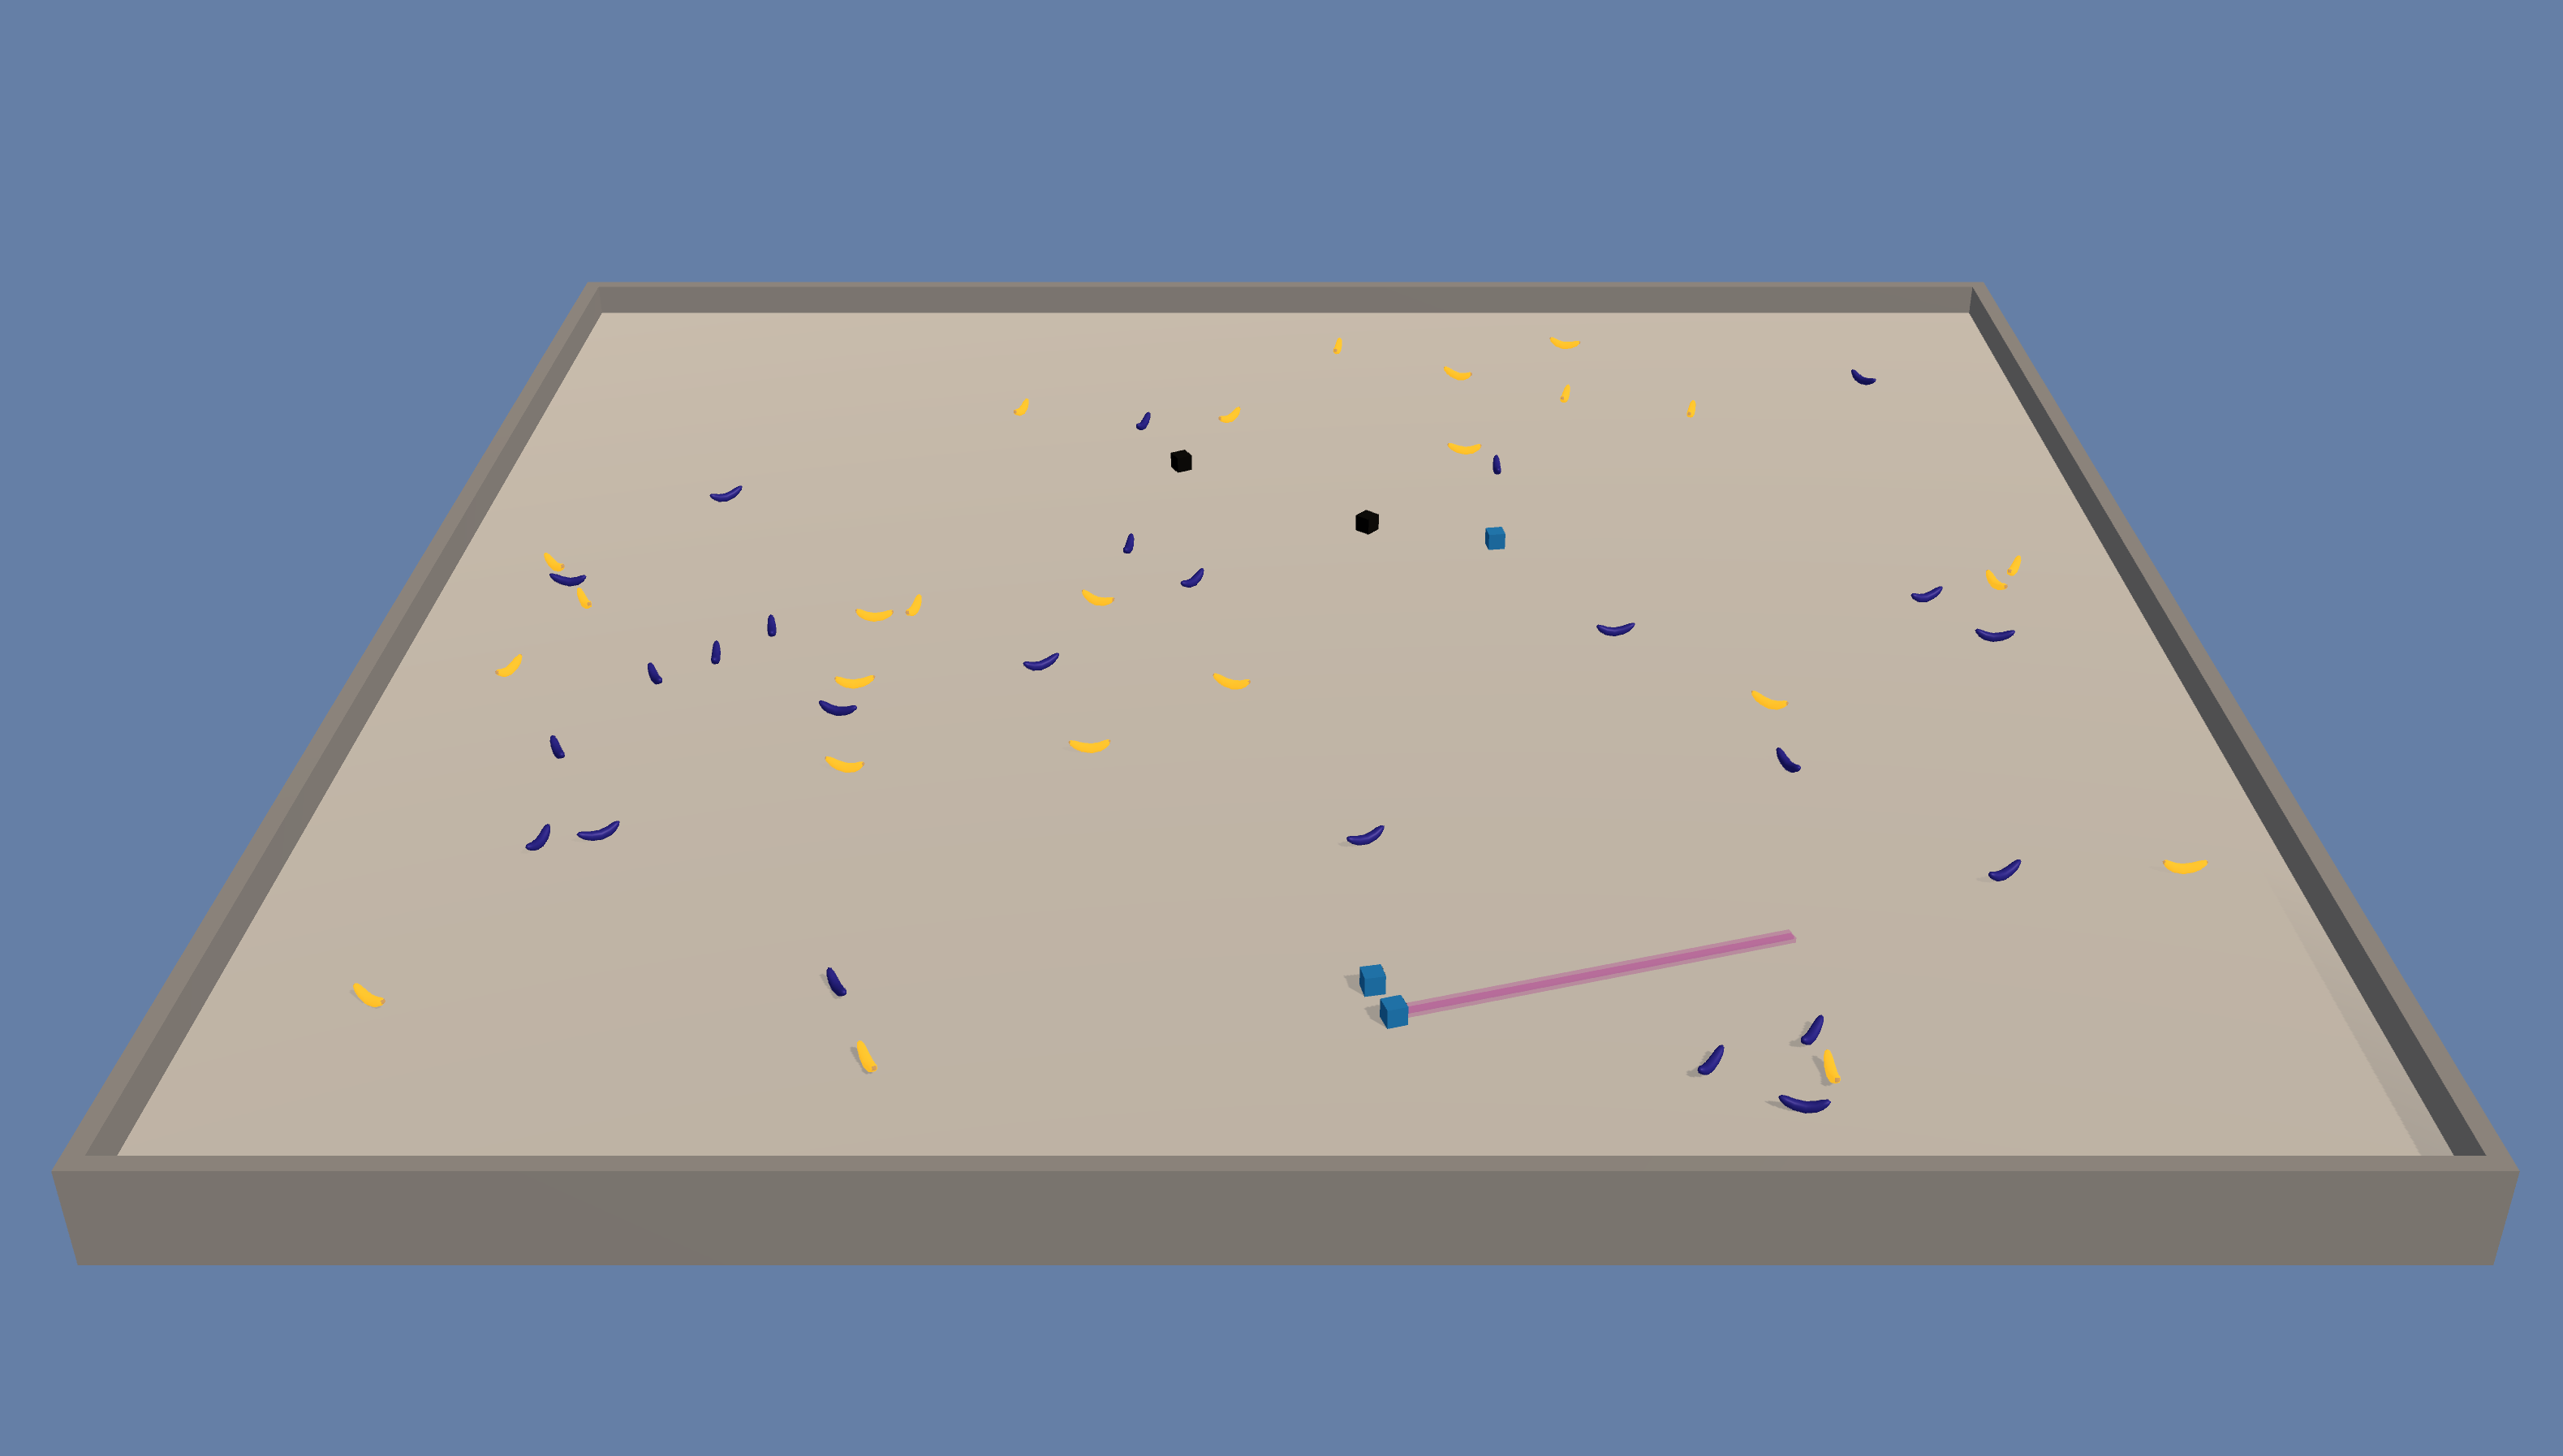
\includegraphics[height=1.5in]{images/banana.png}
   \caption{Unity ML-Agent: Banana Collector}
 }

\maketitle


\keywordlist

%% Required for all content. 

%%%%%%%%%%%%%%%%%%%%%%%%%%%%%%%%%%%%%%%%%%%%%%%%%%%%%%%%%%%%%%
%% Introduction                                                                                                                             %%
%%%%%%%%%%%%%%%%%%%%%%%%%%%%%%%%%%%%%%%%%%%%%%%%%%%%%%%%%%%%%%
\section{Introduction}

In this project I'll present the following three solutions to the  
\href{http://github.com/Unity-Technologies/ml-agents/blob/master/docs/Learning-Environment-Examples.md#banana-collector}{\underline{Unity ML-Agent Banana Collector environment}}:
\begin{enumerate}
	\item {\em Deep Q-Learning}~\cite{DBLP:journals/nature/MnihKSRVBGRFOPB15},
	\item {\em Double Deep Q-Learning}~\cite{DBLP:journals/corr/HasseltGS15}, and
	\item {\em Dueling Deep Q-Learning}~\cite{DBLP:journals/corr/WangFL15}. 
\end{enumerate}
Source code in Python, using PyTorch, is available on 
\href{http://github.com}{\underline{github}} 
in the repo 
\href{http://github.com/bobflagg/Deep-Q-Learning-for-Navigation}{\underline{Deep-Q-Learning-for-Navigation}}.
%%%%%%%%%%%%%%%%%%%%%%%%%%%%%%%%%%%%%%%%%%%%%%%%%%%%%%%%%%%%%%
%% Background                                                                                                                             %%
%%%%%%%%%%%%%%%%%%%%%%%%%%%%%%%%%%%%%%%%%%%%%%%%%%%%%%%%%%%%%%
\section{Background}

The Unity ML-Agent Banana Collector is a {\em sequential decision making problem}, in which an agent interacts with an environment over discrete time
steps and seeks to maximize the expected {\em discounted return}:
$$G_t = \sum_{\tau=t}^{\infty}\gamma^{\tau-t}R_\tau,$$
where $\gamma\in[0,1]$  is a discount factor that trades-off the importance of immediate and future rewards.
See~\cite{DBLP:books/lib/SuttonB98} for a general discussion of this sort of problem. 
In this specific example, the agent observes a 37 dimensional vector containing the agent's velocity, along with ray-based perception of 
objects around the agent's forward direction and tries to learn how to best select one of the following actions:
\begin{enumerate}
	\item move forward,
	\item move backward,
	\item turn left, and
	\item turn right.
\end{enumerate}
A reward of +1 is provided for collecting a yellow banana, and a reward of -1 is provided for collecting a blue banana.
Thus, the goal of the agent is to collect as many yellow bananas as possible while avoiding blue bananas.
%% https://arxiv.org/pdf/1511.06581.pdf

%%%%%%%%%%%%%%%%%%%%%%%%%%%%%%%%%%%%%%%%%%%%%%%%%%%%%%%%%%%%%%
%% Deep Q-Learning for Navigation                                                                                                %%
%%%%%%%%%%%%%%%%%%%%%%%%%%%%%%%%%%%%%%%%%%%%%%%%%%%%%%%%%%%%%%
\section{ Deep Q-Learning for Navigation}

\begin{figure}[h]
	\centering
	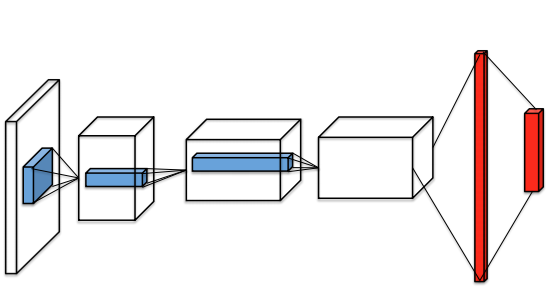
\includegraphics[width=3.0in]{images/dqn}
	\caption{Deep Q-Networt~\protect\cite{DBLP:journals/corr/WangFL15}}
	\label{fig:dqn}
\end{figure}

In deep Q-learning the action-value function, $Q(s,a)$ is approximated with a {\em deep Q-network},
$Q(s,a|\theta)$, with parameters $\theta$.  To train this {\em local network}, we optimize the following sequence
of loss functions at iteration $i$:
$$L_i(\theta_i) = \mathbb{E}\big[\big(y_i^{DQN}-Q(s,a|\theta_i)\big)^2\big],$$
with 
$$ y_i^{DQN}=R_i+\gamma\cdot\max_{a'}Q(s',a'|\theta^-_i),$$
where $\theta^-$ representes the parameters of a fixed and separate {\em target network}.

\FloatBarrier
\begin{figure}[h]
	\centering
	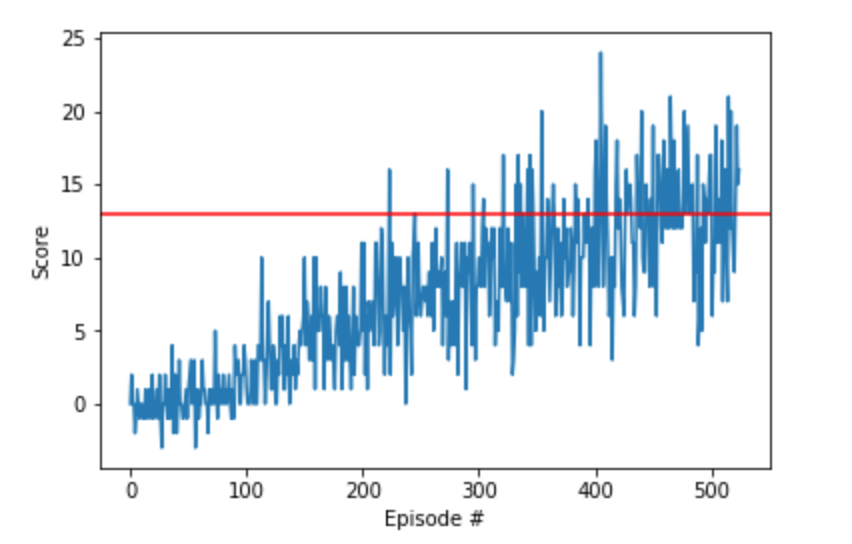
\includegraphics[width=3.0in]{images/dqn-scores}
	\caption{Scores for Deep Q-Learning}
	\label{fig:ferrari}
\end{figure}
\FloatBarrier

%%%%%%%%%%%%%%%%%%%%%%%%%%%%%%%%%%%%%%%%%%%%%%%%%%%%%%%%%%%%%%
%% Deep Q-Learning for Navigation                                                                                                %%
%%%%%%%%%%%%%%%%%%%%%%%%%%%%%%%%%%%%%%%%%%%%%%%%%%%%%%%%%%%%%%
\section{ Double Deep Q-Learning for Navigation}

In Q-learning and deep Q-learning, the max operator uses the same values to both select and evaluate an action. 
This can lead to over optimistic value estimates.  {\em Double deep Q-learning} mitigates this problem by using a different target:
$$ y_i^{DDQN}=R_i+\gamma\cdot Q(s',  \operatorname{arg\,max}_{a'} Q(s',a'|\theta_i)|\theta^-).$$

\begin{figure}[h]
	\centering
	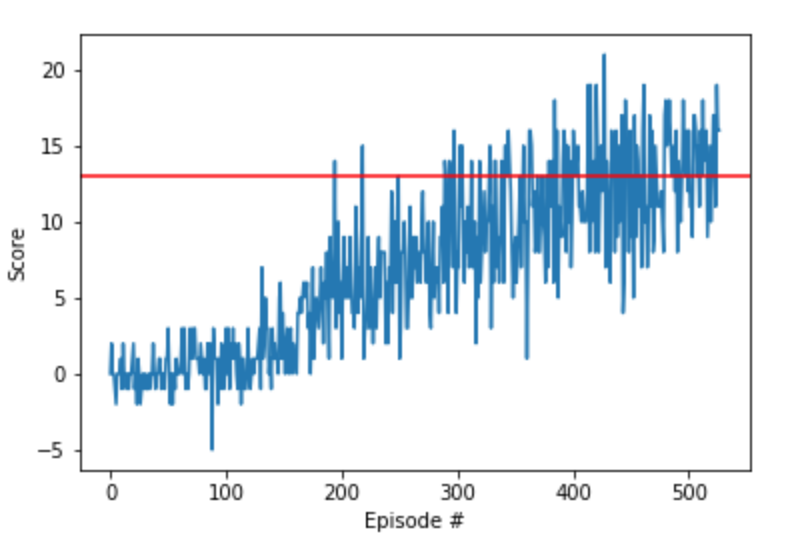
\includegraphics[width=3.0in]{images/double-dqn-scores}
	\caption{Scores for Double Deep Q-Learning}
	\label{fig:ferrari}
\end{figure}

%%%%%%%%%%%%%%%%%%%%%%%%%%%%%%%%%%%%%%%%%%%%%%%%%%%%%%%%%%%%%%
%% Deep Q-Learning for Navigation                                                                                                %%
%%%%%%%%%%%%%%%%%%%%%%%%%%%%%%%%%%%%%%%%%%%%%%%%%%%%%%%%%%%%%%
\section{ Dueling Deep Q-Learning for Navigation}

\begin{figure}[h]
	\centering
	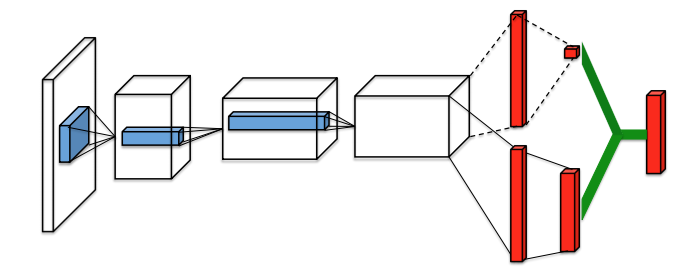
\includegraphics[width=3.0in]{images/dueling-dqn}
	\caption{Dueling Deep Q-Network~\protect\cite{DBLP:journals/corr/WangFL15}}
	\label{fig:ferrari}
\end{figure}

The architecture of the Q-network in dueling deep Q-learning has two streams, one estimates the state-value function, $V(s|\theta, \beta)$, and the other estimates an {\em advantage function},
which in one implementation has the form
$$A(s,a|\theta, \alpha) - \frac{1}{{\cal |A|}}\sum_{a'}A(s, a'|\theta, \alpha).$$
The estimate of the action-value function is then
$$Q(s,a|\theta, \alpha, \beta) = V(s|\theta, \beta) - \big(A(s,a|\theta, \alpha) - \frac{1}{{\cal |A|}}\sum_{a'}A(s, a'|\theta, \alpha)\big).$$

{\bf Note:} I don't use convolution in the network for the Unity ML-Agent Banana Collector so there are no shared $\theta$ parameters in this example.

\begin{figure}[h]
	\centering
	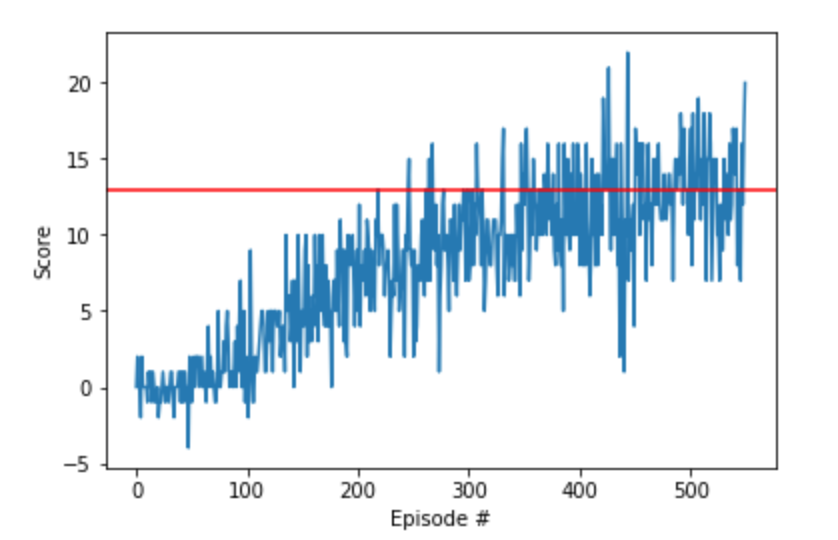
\includegraphics[width=3.0in]{images/dueling-dqn-scores}
	\caption{Scores for Dueling Double  Deep Q-Learning}
	\label{fig:ferrari}
\end{figure}


%%%%%%%%%%%%%%%%%%%%%%%%%%%%%%%%%%%%%%%%%%%%%%%%%%%%%%%%%%%%%%
%% Deep Q-Learning for Navigation                                                                                                %%
%%%%%%%%%%%%%%%%%%%%%%%%%%%%%%%%%%%%%%%%%%%%%%%%%%%%%%%%%%%%%%
\section{Improving Performance}





\bibliographystyle{acmsiggraph}
%\bibliographystyle{abbrv}
%%\nocite{*}
\bibliography{main}
\end{document}